\section{Gruppenantennen}\label{sec:gruppenantennen}
Der Dipol ist ein Rundstrahler, da die Strahlung keine bevorzugte Richtung in der Ebene senkrecht zur Antennenachse aufweist. Bei Punkt-zu-Punkt Verbindungen kann die Reichweite der Antenne bei unveränderter Energie erheblich vergrössert werden, wenn eine Richtwirkung vorhanden ist. Mit der Richtwirkung lässt sich der Störabstand verbessern, da mögliche Störquel-len durch die Richtcharakteristik zum Teil ausgeblendet werden. Eine gewünschte Richtwirkung kann durch Kombination zweier oder mehrerer Dipole mittels Interferenz der Feldstärken erzeugt werden.\\

Die folgenden Betrachtungen basieren auf dem linearen Superpositionsprinzip. Dies geht davon einer ungestörten Überlagerung der Strahlungsbeiträge aller Teilstrahler aus. Das Maximum des resultierenden Feldes befindet sich dort, wo die Felder der Einzelstrahler phasengleich schwingen. Die Felder der Einzelstrahler, die ausserhalb der Hauptstrahlungsrichtung sind, löschen sich gegenseitig mehr oder weniger aus. Die Richtwirkung kann mit diesen Faktoren beeinflusst werden.

\begin{itemize}
	\item Anzahl Strahler
	\item Anordnung der Strahler
	\item Stromamplitude der einzelnen Strahler
	\item Phasenverschiebung der einzelnen Strahler
\end{itemize}

In der Abbildung \ref{fig:gruppenantennen} sind drei unterschiedliche Formen von Gruppen aus Dipolantennen die sich für die Nachrichtenübertragung bewährt haben. 

\begin{figure}[H]
	\centering
	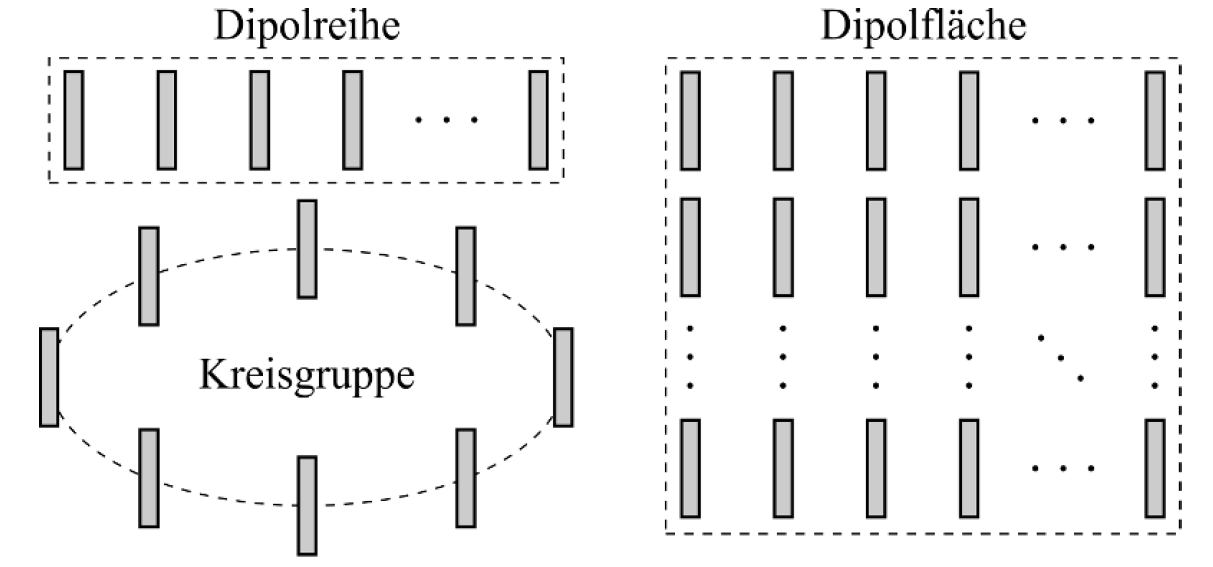
\includegraphics[width=0.75\linewidth]{gruppenantennen}
	\caption{Anordnung von Einzelstrahlern zu einer Antennengruppe.}\label{fig:gruppenantennen}
\end{figure}

Bei Strahlergruppen mit bauartgleichen Teilantennen in gleicher räumlicher Ausrichtung lässt sich das Fernfeld als Produkt von zwei Faktoren schreiben. Der erste Faktor ist die Einzelcharakteristik $ C_{E} $ und beschreibt das Fernfeld des einzelnen Antennenelementes. Die Gruppencharakteristik $ C_{Gr} $ ist der zweite Faktor. Er ist unabhängig von der Art des Einzelstrahlers und beschreibt das Zusammenwirken der Strahler. Unter der Voraussetzung dass die Entfernung des Aufpunktes im Fernfeld gross gegen die räumlichen Abmessungen des Antennensystems aus mehreren Einzelstrahlern und gross gegen die Wellenlänge $ \lambda_{0} $ so können die beiden Faktoren multipliziert werden. Dies ergibt die nachfolgende Formel.

\begin{equation}
C_{ges}=C_{Gr}C_{E}
\end{equation}


\subsection{Querstrahler}\label{sec:querstrahler}

Der Querstrahler gehört zu den linearen Gruppenstrahler und ist eine Dipolzeile, welche in der Abbildung \ref{fig:dipolzeile} dargestellt ist. Bei dieser Gruppe stehen die Dipole senkrecht zur Standlinie (y-Achse).\\

Beim Querstrahler ist die Gruppencharakteristik rotationssymmetrisch zur Gruppenachse. Sie entsteht indem alle Einzelstrahler gleichphasig $ \delta = 0$ erregt werden. Denn dann sind in der Mittelsenkrechten zur Gruppenachse ihre sämtlichen Feldanteile in Phase. Zusätzlich muss der Elementabstand $ a < \lambda_{0} $ sein, damit der Hauptanteil der Energie senkrecht zur Gruppenachse in einen scheibenförmigen Sektor ausgestrahlt wird und weitere Hauptkeulen nicht auftreten können. 

\begin{figure}[H]
	\centering
	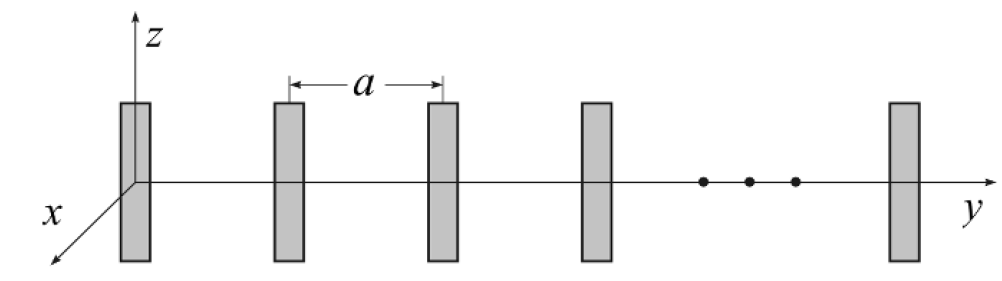
\includegraphics[width=0.75\linewidth]{dipolzeile}
	\caption{Anordnung von baugleichen, äquidistanten Einzelstrahlern zu einer Horizontaler Dipolzeile.}\label{fig:dipolzeile}
\end{figure}

\subsection{Simulation}

Für die Simulation ist eine querstrahlende Dipolzeile mit zwei Einzelstrahler, wie in der Abbildung \ref{fig:querstrahler} aufgebaut worden. Der Dipolabstand beträgt $ a = 2\lambda_{0} $. Dieser führt bei einfacher Speisung zu einer guten Querabstrahlung bei kleinen Nebenkeulen. 

\begin{figure}[!ht]
	\centering
	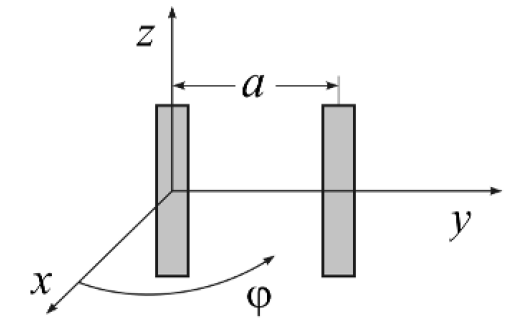
\includegraphics[width=0.5\linewidth]{querstrahler}
	\caption{Aufbau des Querstrahlers.}\label{fig:querstrahler}
\end{figure}

Die Gruppencharakteristik für zwei Strahlerelemente lässt sich mit der Formel einer linearen Gruppe wie folgt berechnen:

\begin{equation}
C_{Gr}(\vartheta,\varphi) = \left|  \cos \left( \dfrac{\sin(N u/2)}{N \sin(u/2)}  \right) \right| = \left|  \cos \left( \dfrac{\sin(u)}{2 \sin(u/2)}  \right) \right|.
\end{equation}

Diese Formel lässt sich vereinfachen und erhält dieses Resultat:

\begin{equation}
C_{Gr}(\vartheta,\varphi) = \left|  \cos \left( \dfrac{k_{0} a}{2} \sin \vartheta \sin\varphi \right) \right|.
\end{equation} 

Das horizontale Richtdiagramm erhält man für $ \vartheta = \pi / 2 $:

\begin{equation}
C_{Gr}^{H}(\varphi) = \left|  \cos \left( \dfrac{\pi a}{\lambda_{0}} \sin \varphi \right) \right|.
\end{equation} 

\begin{figure}[!ht]
	\centering
	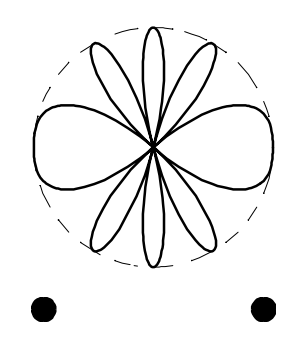
\includegraphics[width=0.4\linewidth]{2Lambda.png}
	\caption{Direktivität des Antennenarrays mit einem Abstand von $2\lambda_0$.}\label{fig:2Lambda}
\end{figure}

In Abbildung \ref{fig:2Lambda} ist das Richtdiagramm für zwei Dipole mit dem Abstand $2\lambda_0$ zu sehen. Dies ist das erwünschte Resultat der Simulation.

\newpage

\begin{figure}[!ht]
	\centering
	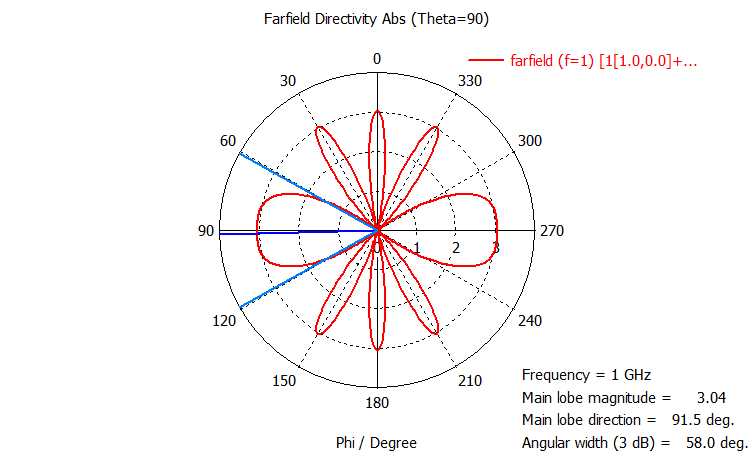
\includegraphics[width=\linewidth]{Array.png}
	\caption{Simulation des Antennenarrays mit $a = 2\lambda_0$.}\label{fig:Array}
\end{figure}

In der Abbildung \ref{fig:Array} ist das Richtdiagramm grafisch dargestellt. Die Anzahl der Nebenkeulen und auch die Form des Richtdiagrammes stimmen mit dem erwarteten Plot überein, weshalb die Simulation als erfolgreich angesehen werden kann. Was jedoch beachtet werden muss, ist dass durch die Abstrahlcharakteristik das Richtdiagramm bei einem konstanten Winkel von $\vartheta$ ausgewertet werden muss, welcher \SI{90}{\degree} beträgt.